\section{The Data Cleaning Library}
 In this section, we describe the architecture and API of the data cleaning library. 
 
\begin{figure}
\centering
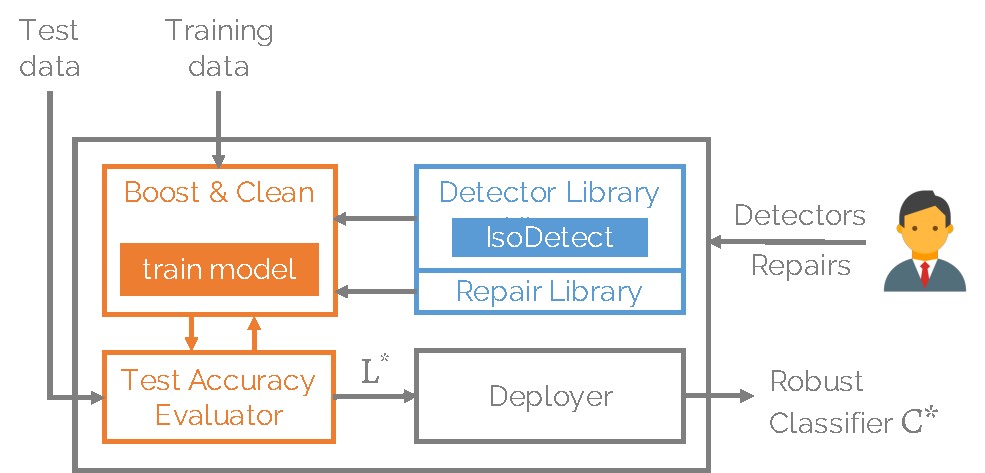
\includegraphics[width=0.8\columnwidth]{figures/arch.pdf}
\caption{\sys system architecture.}
\label{f:arch}
\end{figure}

\subsection{Architecture}
The architecture of \sys includes three high-level components: (1) a loader, (2) error detector, and (3) repair action selector.
The loader takes in a weakly structured dataset (e.g., a CSV file) parses the file and returns a relation over a set of attributes and associated data types with each attribute.
Then, this relation is passed into an error detector.
The error detector identifies a candidate set of erroneous records and taxonomizes them into group of violated constraints.
Finally, associated with each of the violated constraint are repair actions (described in Section 3).
This modular architecture allows us to build a large number of library components, where users can specify additional rules for error detection without having to specify repair actions.
This section will overview the architecture of each of the components (including error detection) and the next section will go into the implementation details of the error detection module.

\subsection{Error Detection}
We noticed that many derived rules follow a similar structure.
First, they convert a row into a feature vector (in the above example, trivially projecting onto $num\_employees$).
Next, they apply a threshold (possibly multi-dimensional) on the feature vector.
We propose a modular architecture that has a single outlier detection technique (called Isolation Forests) at the end of the pipeline but allows for different types of featurization.
User defines a function that maps a row to a vector in $\mathbb{R}^d$ and the Isolation Forest identifies outliers in this space.
For a scalar feature in $\mathbb{R}$, the Isolation Forest degenerates into a threshold rule. 
We experimented with alternative outlier detection techniques (e.g., Minimum Covariance Determinant) but found that the Isolation Forest provided the best tradeoff between runtime and accuracy.

While the availability of such rules is a typical assumption in data cleaning~\cite{DBLP:conf/sigmod/ChuIKW16},  defining such rules requires extensive domain knowledge and is time-consuming.
One of our design objectives is to minimize the burden on data scientists, so we provide an initial library of rules which are described in the next section.
These rules are not meant to replace domain knowledge but rather to address routine problems seen across many different datasets.



\subsection{Loader}
The first step in using \sys is loading a dataset. \sys requires that that data is initially weakly structured, similar to the assumptions of SQLShare~\cite{howe2013sqlshare}. It assumes that each row corresponds to a record and attributes are delimited, but there are potentially missing values, the domain of possible attribute values are unknown, and the data types are unknown.
We implemented a schema-on-read loading module that takes as input a SQL table, CSV, or a text file.
This module returns a structured relation of tuples and inferred data types for each attribute (numerical, categorical, string, date, address).
We designed the type inference to be soft--allowing for errors to exist in the dataset.
The module automatically builds indices over the numerical and categorical attributes.
These indices will help optimize the error detection module.



\subsection{Cleaner}
Given a set of detected violations $\{V_1,...,V_j\}$, the cleaner assigns a tuple possible repair action to each $V_i$ (one if the data is in training, one if the data is in test).
Repairs are applied as a batch to each set of violations and not in a per-cell basis.
The available options are:
\begin{enumerate}
    \item \emph{Impute the mean (Train and Test): } Impute a cell in violation with the mean value of the attribute calculated over the training data excluding violated cells.
    \item \emph{Impute the mode (Train and Test): } Impute a cell in violation with the most frequent value of the attribute calculated over the training data excluding violated cells.
    \item \emph{Impute the median (Train and Test): }Impute a cell in violation with the median value of the attribute calculated over the training data excluding violated cells.
     \item \emph{Discard (Train Only): } Discard a row with a violated cell from the training dataset.
     \item \emph{Fail-Safe (Test Only): } Automatically predict the most-frequent label for a row with a violated cell.
\end{enumerate}

The cleaner's role is to learn an assignment of these actions to each of the violations.
The combination of the actions and the predicates define the data cleaning libary $\mathcal{L}$.







